\chapter{波动光学3(偏振)}
\section{选择题}
\exercise B

\solve 由马吕斯定律知,线偏光透过检偏器时的光强$I=I_0\mathrm{cos}^2\theta$,故光强先增加,后减小至0。

\exercise D

\solve A:部分偏振光可以看作是线偏光和自然光的合成,而自然光的光振动沿任意方向都有分布,正确;

B:部分偏振光的自然光分量透过旋转的偏振片永远不会使光强降为0,正确;

C:自然偏振光和线偏光均可以分解为两个相互正交的、无相位关系的线偏光,正确;

D:部分偏振光中的自然光分量在经过偏振片时光强一定会减小,错误,选D。

\exercise C

\solve 从偏振度的定义来看,图中两个方向偏振的光的标记数量得越均匀,则偏振度越小。其中C图两个方向偏振的光的标记数量相等,是自然光,故偏振度为0,偏振度最小,选C。

\exercise C

\solve 如果入射光是部分偏振光,则在偏振光旋转的时候,部分偏振光的线偏振光部分的光强会变化,而自然偏振光部分不会变化,叠加起来导致出射光强对偏振片转动有变化但没有消光,满足条件;

如果是椭圆偏振光,则可根据椭圆的对称轴将偏振光分解为正交的两个分量$I_1\leqslant I_2$,总光强$I_0=I_1+I_2$,如图\ref{4}所示。

\begin{figure}[htbp]
	\centering
	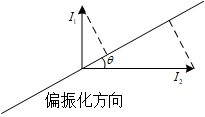
\includegraphics[scale=0.9]{Chp17_4.jpg}
	\caption{题4 示意图}
	\label{4}
\end{figure}

其中在经过偏振片后,透过两线偏光光强分别为$I_1'=I_1\mathrm{sin}^2\theta$,$I_2'=I_2\mathrm{cos}^2\theta$。而$I_1',I_2'$原本d的相位差为$\frac{\pi}{2}$或$\frac{3\pi}{2}$,在有些时候,当偏振方向使得矢量在相反方向分解时,有附加相位差$\pi$,故总的相位差仍可化为$\Delta \varphi=\frac{\pi}{2},\frac{3\pi}{2}$。而两线偏光在同一偏振面内,故合成的是线偏光,光强为$I=I_1'+I_2'+2\mathrm{cos}\Delta \varphi\sqrt{I_1'I_2'}$,代入上述关系,得$I=I_1\mathrm{sin}^2\theta+I_2\mathrm{cos}^2\theta=I_1+(I_2-I_1)\mathrm{cos}^2\theta$。当$I_1\not= I_2$时,$I$会随$\theta$变化,且$I_2-I_1>0$,光强不会变为0,不会消光,这种椭圆偏振光满足条件;而当$I_1=I_2$时,即圆偏光,$I=I_1=I_2=\frac{1}{2}I_0$,光强与偏振片角度无关,即光强不变化,故圆偏光一定不满足条件。

如果入射光是线偏光,则当偏振化方向与偏振方向垂直时会消光,不满足条件。

由以上讨论对选项进行检查:A,B:入射光是部分偏振光或是非圆偏光的椭圆偏振光时,可以满足条件,故两者都错;C:入射光是圆偏光时,偏振光旋转不可能使光强发生变化,故不可能是圆偏光,正确;D:旋转偏振片可以使线偏光消光,错误。

\exercise A

\solve 在光经过偏振片后,光的强度减为原来的一般,而光的偏振方向相同,仍然满足干涉条件,故在屏上仍有干涉条纹,但光强减为原来的一半,选A。

\exercise B

\solve 由书中介绍,可以得知自然光入射到两种介质界面上时,反射光一般是部分偏振光,在入射角为布儒斯特角时反射光为线偏光。故ACD正确,B错误。

\exercise B

\solve 由于自然光是以布儒斯特角从空气入射玻璃,故1光是线偏振光,2光是部分偏振光;而2光从玻璃入射空气时,也是以布儒斯特角入射,故反射光3是线偏振光,且光矢量方向垂直于入射面,选B。

\exercise C

\solve 由书中对o光和e光的介绍,知o光在晶体中的波阵面是球面,e光在晶体中的波阵面是旋转椭球面,选C。

\exercise C

\solve 见题4对椭圆偏振光透过偏振片的光强的推导,有当椭圆偏振光为圆偏光时,透过的线偏光的光强为$I=\frac{1}{2}I_0$,是原来光强的一半。故选C。

\exercise A

\solve 自然光可以沿1/4波片的光轴方向分解为两个光强相等的正交分量,但没有固定的相位关系,故在通过波片后,虽然某一方向的相位增加了$\frac{\pi}{2}$,但两分量的相位差仍然没有固定关系,但两分量的光强度不变,所以出射光仍然是自然光,选A。

\section{填空题}

\exercise 起偏方向$\quad$起偏器$\quad$检偏器

\solve 由书中定义可得。

\exercise 平行于入射面

\solve 已知以布儒斯特角入射的光线,其反射光只能是垂直于入射面的;而由于这束偏振光没有反射的部分,故该偏振光没有垂直于入射面的分量,故该偏振光的光矢量振动方向为平行于入射面。

\exercise $\frac{\sqrt{2}}{2}A$

\solve 将振幅沿偏振光方向分解,沿偏振方向的振幅为$A'=A\mathrm{cos}45^{\mathrm{o}}=\frac{\sqrt{2}}{2}A$,故透过偏振片的光振幅为$\frac{\sqrt{2}}{2}A$。

\exercise $60^{\mathrm{o}}$

\solve 自然光透过第一个偏振片后光强变为$I'=\frac{1}{2}I_0$,变为线偏光,再经过第二个偏振片后光强变为$I=I'\mathrm{cos}^2\theta=\frac{1}{2}\mathrm{cos}^2\theta I_0$,其中$\theta$为两偏振片的夹角。又知$I=\frac{1}{8}I_0$,故有$\frac{1}{2}\mathrm{cos}^2\theta=\frac{1}{8}$,取$0\leqslant\theta\leqslant 90^{\mathrm{o}}$,有$\theta=60^{\mathrm{o}}$。

\exercise 线偏光$\quad$垂直于入射面$\quad$部分偏振光

\solve 由书中对布儒斯特角的介绍可得。

\exercise $\mathrm{arctan}\frac{n_2}{n_1}$

\solve 入射角为$i_B$(布儒斯特角)时,折射角为$\gamma=\frac{\pi}{2}-i_B$。又由折射关系,知$n_1\mathrm{sin}i_B=n_2\mathrm{sin}\gamma=n_2\mathrm{cos}i_B$,故$\mathrm{tan}i_B=\frac{n_2}{n_1}$,有$i_B=\mathrm{arctan}\frac{n_2}{n_1}$。

\exercise $\frac{1}{2}I$

\solve 由题4对椭圆偏振光中特殊情况圆偏光的分析可得。

\exercise o$\quad$e

由书中对双折射现象的介绍可得。

\exercise $5\times 10^{-6}\mathrm{m}$

\solve 由o光和e光在材料中不同的折射率,得材料中o光和e光的光程差为$\Delta=d|n_o-n_e|$,其中$d$为材料的厚度;当$\Delta=\frac{\lambda}{4}+k\lambda,k=0,1,2,\cdots$时,可以变为1/4波片。为使$d$最小,取$k=0$,得$d_{\mathrm{min}}=\frac{\lambda}{4|n_e-n_o|}=5\times 10^{-6}\mathrm{m}$。

\exercise 在光路中添加1/2波片

\solve 将右旋椭圆偏振光沿波片的光轴分解为正交的两个振动分量,假设分解如图\ref{fig:17_20}中方向所示。

\begin{figure}[htbp]
	\centering
	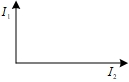
\includegraphics[scale=0.9]{Chp17_20.jpg}
	\caption{题20 示意图}
	\label{fig:17_20}
\end{figure}

由于偏振光右旋,故$I_2$方向的偏振超前$I_1$方向$\Delta \varphi\leqslant\frac{\pi}{2}$;在通过半波片后,$I_2$方向的偏振超前$I_1$方向$\Delta \varphi\pm\pi$,均可等效为$\Delta \varphi'=\Delta \varphi-\pi$,其中$-\frac{\pi}{2}\leqslant\Delta \varphi'\leqslant0$,可理解为$I_1$超前$I_2$的相位为$-\Delta \varphi'=\pi-\Delta \varphi$,则方向变为右旋。故可以通过加1/2波片使椭圆偏振光从右旋变成左旋。

\section{计算题}
\exercise 

\solve 设部分偏振光的自然光部分的光强为$I_1$,线偏光部分的光强为$I_2$。在偏振片移动到透射光强最大位置时,偏振化方向与线偏光相同,则透射光强为$I_{\mathrm max}=\frac{1}{2}I_1+I_2$;当偏振片旋转$60^{\mathrm{o}}$时,透射光强为$I=\frac{1}{2}I_1+I_2\mathrm{cos}^260^{\mathrm{o}}$。由题中所给关系$I=\frac{1}{2}I_{\mathrm max}$,解得$I_1:I_2=1:1$。

\exercise $45^{\mathrm{o}}$

\solve 设第二个偏振片和第一个偏振片的夹角为$\theta$,则第二个偏振片和第三个偏振片的夹角为$90^{\mathrm{o}}-\theta$。则有透射光光强为$I=\frac{1}{2}I_0\mathrm{cos}^2\theta\mathrm{cos}^2(90^{\mathrm{o}}-\theta)=\frac{1}{2}I_0\mathrm{cos}^2\theta\mathrm{sin}^2\theta=\frac{1}{8}I_0\mathrm{sin}^22\theta$。则当$\theta=45^{\mathrm{o}}$时,光强最大。

\exercise $I'=\frac{5}{8}I_0$$\quad$$I''=\frac{5}{32}I_0$

\solve 入射光为强度相等的线偏振光和自然偏振光混合而成,故线偏光部分强度为$I_1=\frac{1}{2}I_0$,自然光部分强度为$I_2=\frac{1}{2}I_0$。在该光经过第一个偏振片时,光强变为$I'=I_1\mathrm{cos}^2 30^{\mathrm{o}}+\frac{1}{2}I_2=\frac{5}{8}I_0$,为线偏光。再经过第二个偏振片,光强变为$I''=I'\mathrm{cos}^2 60^{\mathrm{o}}=\frac{5}{32}I_0$。

\exercise $1.28\mathrm{\mu m}$

\solve 设晶片的厚度为$d$。光的分解和叠加情况如图\ref{24}所示。

\begin{figure}[htbp]
	\centering
	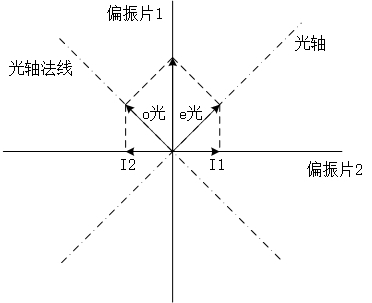
\includegraphics[scale=0.6]{Chp17_24.jpg}
	\caption{题24 示意图}
	\label{fig:17_24}
\end{figure}

从图\ref{fig:17_24}中可以看出,在自然光经过偏振片1后,变为线偏光;在经过方解石晶片后被分解为o光和e光,并且由于其在晶片中的运动速度不同,产生了一部分光程差;再经过偏振片2,o光和e光均被分解到偏振片2的方向($I_1,I_2$)。可以看出,其参考方向相反,则在干涉叠加的时候又附加光程差$\frac{\lambda}{2}$。故$I_1,I_2$之间总光程差为$\delta=d|n_o-n_e|+\frac{\lambda}{2}$。而当$\delta=n\lambda,n=1,2,\cdots$时,光达到相长干涉,光通过系统达到极大。则计算得满足条件的$d=\frac{\lambda}{|n_o-n_e|}n-\frac{\lambda}{2|n_o-n_e|}=3.488n-1.744(\mathrm{\mu m})$。

当$n=3$时,$d=8.720 \mathrm{\mu m}<10 \mathrm{\mu m}$;
当$n=4$时,$d=12.208 \mathrm{\mu m}>10 \mathrm{\mu m}$。
故$d$取$8.720 \mathrm{\mu m}$,
应至少磨去$\Delta d=10-8.720=1.28 \mathrm{\mu m}$(保留三位有效数字)。
